\setcounter{figure}{0}

\section{16th July 2023: The God of second chances}
\subsection*{Text: Jonah 3}
  \begin{quote}
    [1] Then the word of the LORD came to Jonah the second time, saying, [2] “Arise, go to Nineveh, that great city, and call out against it the message that I tell you.” [3] So Jonah arose and went to Nineveh, according to the word of the LORD. Now Nineveh was an exceedingly great city, three days’ journey in breadth. [4] Jonah began to go into the city, going a day’s journey. And he called out, “Yet forty days, and Nineveh shall be overthrown!” [5] And the people of Nineveh believed God. They called for a fast and put on sackcloth, from the greatest of them to the least of them.

    [6] The word reached the king of Nineveh, and he arose from his throne, removed his robe, covered himself with sackcloth, and sat in ashes. [7] And he issued a proclamation and published through Nineveh, “By the decree of the king and his nobles: Let neither man nor beast, herd nor flock, taste anything. Let them not feed or drink water, [8] but let man and beast be covered with sackcloth, and let them call out mightily to God. Let everyone turn from his evil way and from the violence that is in his hands. [9] Who knows? God may turn and relent and turn from his fierce anger, so that we may not perish.”

    [10] When God saw what they did, how they turned from their evil way, God relented of the disaster that he had said he would do to them, and he did not do it.
  \end{quote}
\subsection*{Notes}
\begin{itemize}
  \item{Recap:
  \begin{enumerate}
    \item{It is silly to run away from God.}
    \item{It is silly to limit God’s love only to Israel.}
    \item{We saw that when Jonah was sinking, he cried out to God for help and deliverance, and God delivered Jonah out of His mercy.}
  \end{enumerate}}
  \item{Two points:
  \begin{enumerate}
    \item{God gave Jonah a second chance}
    \item{God gave the ninevites a second chance}
  \end{enumerate}}
  \item{Firstly, we see how God gave Jonah a second chance. We see this by how God sent Jonah to Nineveh a second time after rescuing him. God also did not rake up the first failure, He did not keep harping on Jonah’s disobedience. God forgives, and forgets, unlike us humans… we must learn to forgive AND forget, so that when the same mistake comes up again, we treat it like the first time the mistake is being made.}
  \item{We also see how God forgives in such a deep way such that He still trusts us to do His work despite our mistakes. Two examples other than Jonah: David and Peter. Though these people all had made mistakes, after their repentance, God still trusts them to do His work. This is so unlike us humans, even when we forgive a person, we will always feel biased towards the person. We need to stop doing that!}
  \item{Also, from how God forgives Jonah, we can be assured that despite our failures and shortcomings, God still forgives us and uses us. We don’t need to feel too bad to do God’s work, when we sin and when we fall short.}
  \item{Next, we see how God gave the Ninevites a second chance. Despite Jonah’s short message and half-hearted attempt at preaching to the Ninevites (he only walked one day when the city was three days in breadth), the Ninevites all believed Jonah, and even the king. This showed that God in his grace convicted the hearts of all the Ninevites to recognise their sin and their need for deliverance. Thus, we see that in the end, repentance only comes from God’s Spirit convicting the sinner. Now, two things: as polytheists, how did the Ninevites know which god Jonah was referring to? Most likely, Jonah did tell them about his God too, just that it is not reflected in the text. Next thing, we see from v9 that the king did not know that God would forgive. It is uncertain whether Jonah omitted the message of God’s forgiveness or whether it is just not reflected in the text. }
  \item{Next, we see that the repentance of the Ninevites had very concrete actions. Not only were their hearts broken for their sins, they also turned from their evil ways and their violence. Repentance is not just about feeling bad, it is about turning away from sin and towards God. }
  \item{For the king, in his act of repentance, he came down from his throne, took off his robes, and sat in ashes. This act of self-dethronement is a sign of humility, which is necessary for repentance. This self-dethronement is a picture of the self-denial that is commanded of us, for us to take up our cross and follow Jesus. When we repent, we can no longer be the king of our own lives, but Jesus must be the king of our lives. Jesus is not just our savior, He is our Lord.}
  \item{The book of Jonah served to reprimand Israel. Compare Nineveh’s repentance to Israel’s hard hearts; and this is despite Israel having more prophets being sent to them, and Israel having the Law which daily points out their sins. In today’s context, as Jesus says, “But he answered them, “An evil and adulterous generation seeks for a sign, but no sign will be given to it except the sign of the prophet Jonah. For just as Jonah was three days and three nights in the belly of the great fish, so will the Son of Man be three days and three nights in the heart of the earth. The men of Nineveh will rise up at the judgment with this generation and condemn it, for they repented at the preaching of Jonah, and behold, something greater than Jonah is here.” In synagogues, on Yom Kippur, the story of Jonah is being read to remind the Israelites of what repentance looks like. But yet ironically, the Jews reject Jesus, who is greater than Jonah.}
  \item{Conclusion: God has given us a second chance through Jesus who died in our place so we can be freed. Are we willing to take God’s second chance to others by bringing his message of salvation to them?}
  % \item{\begin{figure}[H]
  %   \centering
  %   % 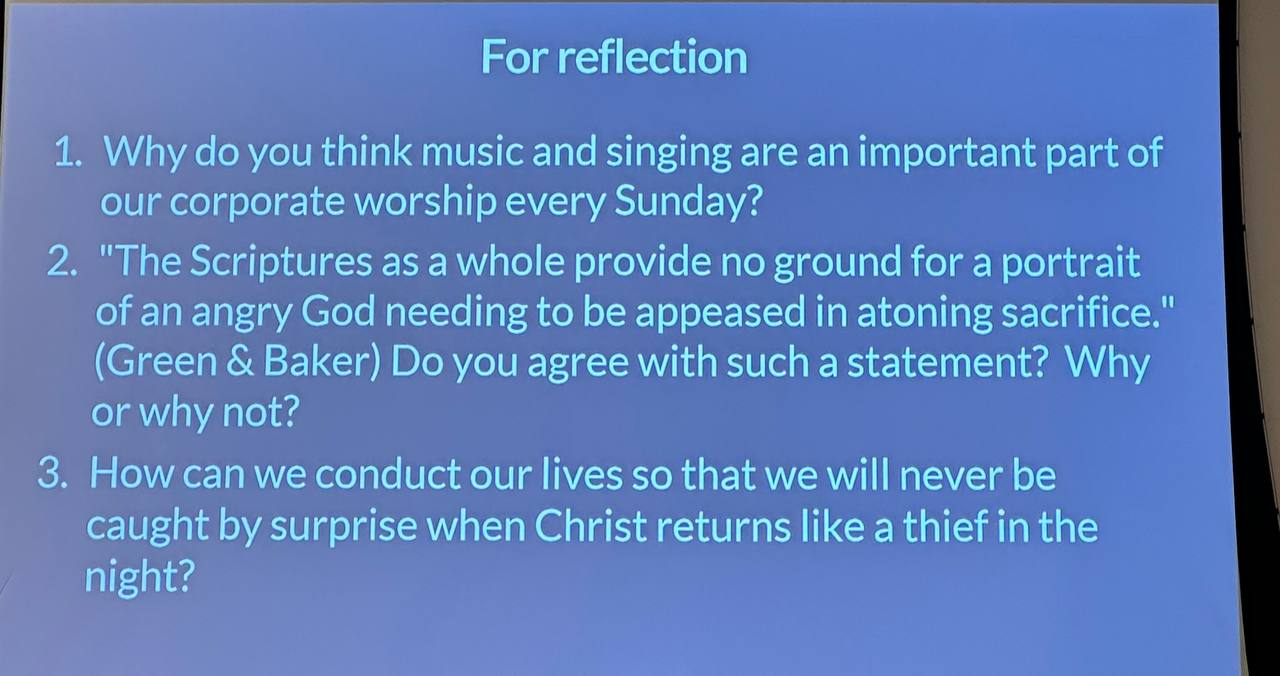
\includegraphics[width=0.8\textwidth, trim={0cm 0cm 0cm 0cm},clip]{Figures/marchSermon4Reflections.jpg}
  %   \includegraphics[width=0.8\textwidth, trim={0cm 0cm 0cm 0cm},clip]{example-image-a}
  %   \caption[]{Reflection questions for this sermon}
  %   \label{}
  % \end{figure}}
\end{itemize}